\documentclass[10,a4paperpaper,]{article}

  \title{Replication Report}
  \author{Primary Replicator\textsuperscript{1}, \and Co-pilot
\textsuperscript{2}}
  \date{%
		\textsuperscript{1} University of someplace\\%
		\textsuperscript{2} University of some other place~\\[2ex]
		\today
   }
  


\newcommand{\iblue}{008080}
\newcommand{\igray}{d4dbde}

\newlength{\cslhangindent}
\setlength{\cslhangindent}{1.5em}
\newenvironment{CSLReferences}%
  {}%
  {\par}

% Author: Karol KozioL
% License: GPL-3
% Modified by: Sarah Wagner & Anna Lohmann

% % % packages -----------------------------------------------------------------------------------
\usepackage{amsmath}
\usepackage{array}
\usepackage{booktabs}
\usepackage{calc}
\usepackage{eso-pic}
\usepackage{fancyhdr}
\usepackage{fontspec}
\usepackage[left = 2.5cm, right = 2.5cm, top = 1.2cm, bottom = 1.2cm, includeheadfoot]{geometry}
\usepackage{graphicx}
\usepackage[utf8]{inputenc}
\usepackage{lastpage}
\usepackage{multirow}
\usepackage{tabularx} 
\usepackage{tikz}
\usepackage{titlesec}
\usepackage{xcolor, colortbl}
\usepackage{url} 
\usepackage[hidelinks]{hyperref} 
\usepackage{pmboxdraw}
\usepackage{placeins}
\usepackage{enumitem}
\usepackage{longtable}
\usepackage{lscape}
%\usepackage{verbatim}
%\makeatletter
%\def\verbatim@font{\scriptsize\ttfamily}
%\makeatother
%\RequirePackage[normalem]{ulem} %DIF PREAMBLE
%\RequirePackage{color}
%\providecommand{\tightlist}{%
%	\setlength{\itemsep}{0pt}\setlength{\parskip{0pt}}
\providecommand{\tightlist}{%
  \setlength{\itemsep}{0pt}\setlength{\parskip}{0pt}}
% % % settings -----------------------------------------------------------------------------------

% % custom colors
\definecolor{iblue}{HTML}{\iblue}
\definecolor{igray}{HTML}{\igray}

% definition of pagename
\newcommand\pagename{Page}

% % fonts 
\defaultfontfeatures{Mapping = tex-text}
\setmainfont[BoldFont = Lato-Bold.ttf, ItalicFont = Lato-Italic.ttf, BoldItalicFont = Lato-BoldItalic.ttf]{Lato-Regular.ttf}
\newfontfamily\headingfont[ItalicFont = Lato-BlackItalic.ttf]{Lato-Black.ttf}
%\setmonofont{Ubuntu Mono}
\setmonofont[Scale=0.90,
BoldFont=UbuntuMono-Bold.ttf,
%ItalicFont=UbuntuMono-Italic.ttf,
BoldItalicFont=UbuntuMono-BoldItalic.ttf
]{UbuntuMono-Regular.ttf}

\makeatletter
\def\verbatim@font{\linespread{1}\normalfont\ttfamily}
\makeatother

% % sections
\titleformat{\section}{\color{iblue}\headingfont\Large\bfseries}{\thesection}{1em}{}[\titlerule]
\titleformat{\subsection}{\color{iblue}\headingfont\large\bfseries}{\thesubsection}{1em}{}
\titleformat{\subsubsection}{\color{iblue}\headingfont\bfseries}{\thesubsubsection}{1em}{}

% % misc
\setlength{\parindent}{0em} 
\linespread{1.5}
\raggedright
\newcolumntype{C}{>{\centering\arraybackslash}X}


\makeatletter

% pagestyle titlepage
\fancypagestyle{customtitle}{
	\lhead{}
	\chead{}
	\rhead{}
	\makeatother
	\lfoot{}
	\cfoot{}
	\rfoot{}
}




% % % header and footer ---------------------------------------------------------------------------
\pagestyle{fancy}
\lhead{}
\chead{}
\rhead{}
\makeatother
\newlength{\myheight}
\lfoot{}
\cfoot{}
\rfoot{\pagename~\thepage \hspace{1pt} / \pageref{LastPage}}
\renewcommand\headrulewidth{0pt}
\renewcommand\footrulewidth{0pt}





\begin{document}


\renewcommand{\contentsname}{Table of Contents}

\renewcommand{\pagename}{Page}


\urlstyle{same}

\maketitle

\subsection*{Abstract}

\texttt{\textless{}a\ summary\ of\ the\ replication\ effort\textgreater{}}
\vskip 2em

\noindent\makebox[\textwidth]{\large Correspondence concerning this replication report should be addressed to:}

\par

\noindent\makebox[\textwidth]{\large primary\_replicator@someuni.edu}

\par

\clearpage

\section{Introduction}

This replication report documents the replication attempt of the
simulation study
\texttt{\textless{}insert\ reference\ of\ replicated\ study\textgreater{}}.
Following the definition of Rougier et al. (2017) we understand the
replication of a published study as writing and running new code based
on the description provided in the original publication with the aim of
obtaining the same results.

\section{Method}

\subsection{Information basis}

\texttt{\textless{}What\ sources\ were\ used\ to\ obtain\ information?\ The\ original\ article,\ some\ appendix,\ online\ supplements,\ other\ articles\ from\ the\ same\ authors,\ code\ available\ from\ the\ authors\ personal\ website?\textgreater{}}

\subsection{Data Generating Mechanism}

Information provided in the above mentioned sources indicated that the
following simulation factors were systematically varied in generating
the artificial data.

\begin{longtable}[]{@{}lll@{}}
\toprule
Simulation factor & No.~levels & Levels \\
\midrule
\endhead
\emph{Varied} & & \\
\emph{Fixed} & & \\
\bottomrule
\end{longtable}

\subsubsection{Simulation Factor 1}

\texttt{\textless{}More\ detail\ of\ how\ factor\ 1\ was\ varied\ and\ implemented\textgreater{}}

\subsubsection{Simulation Factor 2}

\texttt{\textless{}More\ detail\ of\ how\ factor\ 2\ was\ varied\ and\ implemented\textgreater{}}

\subsubsection{Simulation Factor 3}

\texttt{\textless{}More\ detail\ of\ how\ factor\ 3\ was\ varied\ and\ implemented\textgreater{}}

\texttt{\textless{}If\ the\ design\ was\ not\ full-factorial\ describe\ the\ simulation\ scenarios\ by\ other\ means\textgreater{}}

\texttt{\textless{}You\ can\ add\ pseudocode\ or\ a\ flowchart\ to\ illustrate\ the\ data\ generation\ or\ the\ entire\ simulation\ design\textgreater{}}

\begin{minipage}{\linewidth}
Data generation can be summarized with the following pseudo code:

\texttt{For 1000 repetitions of each of 400 unique scenarios:}
\begin{itemize}[leftmargin=*] 
    \item[--] \texttt{Set unique seed based on scenario id and number of repetition.}
    \item[--] \texttt{...}
    \item[--] \texttt{ While some condition < some other condition}
    \begin{itemize}
      \item[$\ast$] \texttt{Sample ... from the given distribution.}
      \item[$\ast$] \texttt{Sample a sample size from the given distribution.}
      \item[$\ast$] \texttt{Compute ... based on these random elements.}
      \item[$\ast$] \texttt{Determine ... based on mechanism of current scenario.}
    \end{itemize}
    \item[--] \texttt{If some condition is > x:}
    \begin{itemize}
      \item[$\ast$] \texttt{Determine ... \& resample from corresponding ... model.}
    \end{itemize}
    \item[--] \texttt{Apply ...}
\end{itemize}
\end{minipage}
\newpage

\FloatBarrier 

\subsection{Investigated Methods}

The study investigates \ldots{}
\texttt{\textless{}Describe\ the\ methods\ that\ are\ investigated\ and\ how\ they\ are\ implemented\textgreater{}}

\subsubsection{Method 1}

\texttt{\textless{}Describe\ how\ the\ first\ method\ is\ defined\ and\ implemented.\ You\ can\ include\ equations\ and\ or\ R\ code.\ If\ applicable,\ mention\ specialized\ R\ packages,\ their\ version\ as\ well\ as,\ parameters\ of\ specific\ functions.\textgreater{}}

\subsubsection{Method 2}

\texttt{\textless{}Describe\ how\ the\ second\ method\ is\ defined\ and\ implemented.\ You\ can\ include\ equations\ and\ or\ R\ code.\ If\ applicable,\ mention\ specialized\ R\ packages,\ their\ version\ as\ well\ as,\ parameters\ of\ specific\ functions.\textgreater{}}

\subsection{Performance measures}

\texttt{\textless{}Describe\ which\ performance\ measures\ are\ compared,\ if\ applicable\ mention\ specialized\ R\ packages,\ their\ versions,\ as\ well\ as\ parameter\ settings\ of\ functions.\textgreater{}}

The following flowchart describes the simulation design

\begin{figure}
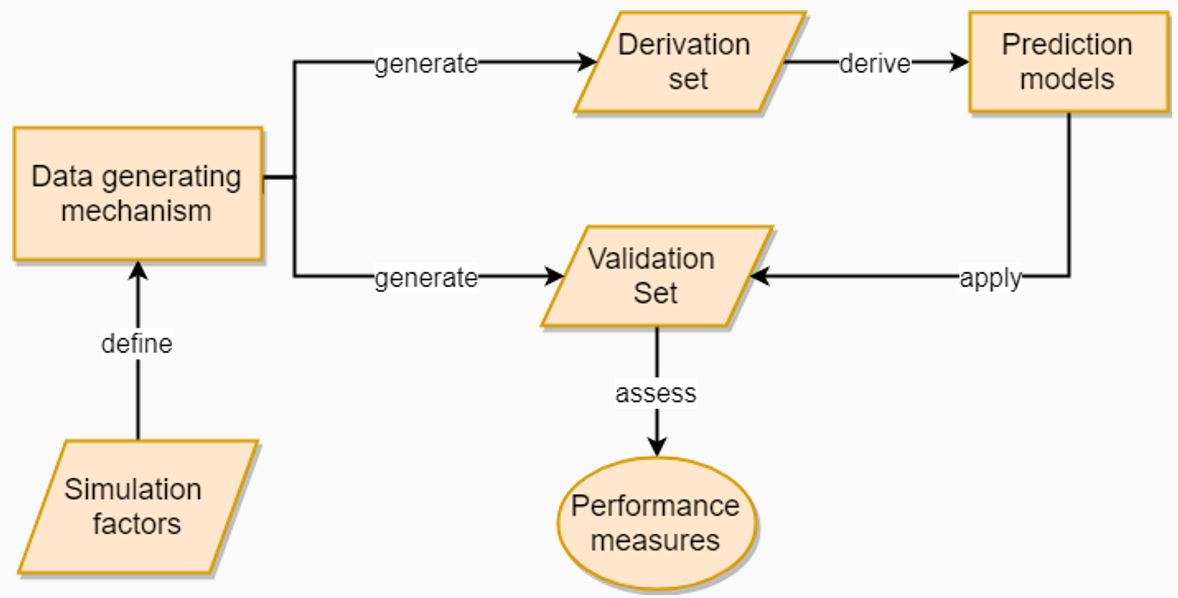
\includegraphics[width=450pt]{flowchart} \caption{Flow chart of data generating mechanism}\label{fig:unnamed-chunk-1}
\end{figure}

\subsection{Technical implementation}

While the original simulation study was carried out in
\texttt{\textless{}computational\ environment\ of\ original\ study\textgreater{}}
our replication was implemented using the R programming environment
(details regarding software versions can be obtained from the section
Reproducibility Information). The corresponding R code can be obtained
from \url{https://github.com/replisims/your_repo}.

The following table provides an overview of replicator degrees of
freedom, i.e.~decisions that had to be made by the replicators because
of insufficient or contradicting information. Issues were resolved by
discussion among the replicators. Decisions were based on what the
replicators perceived to be the most likely implementation with
likeliness estimated by common practice and/or guideline
recommendations. Wherever feasible multiple interpretations where
implemented.

\begin{longtable}[]{@{}
  >{\raggedright\arraybackslash}p{(\columnwidth - 4\tabcolsep) * \real{0.36}}
  >{\raggedright\arraybackslash}p{(\columnwidth - 4\tabcolsep) * \real{0.36}}
  >{\raggedright\arraybackslash}p{(\columnwidth - 4\tabcolsep) * \real{0.27}}@{}}
\toprule
Issue & Replicator decision & Justification \\
\midrule
\endhead
Data dependence & each scenario is implemented in independently
generated data & Best practice (Burton et al. 2006) \\
\bottomrule
\end{longtable}

\subsection{Some issue}

\texttt{\textless{}More\ details\ on\ how\ the\ information\ provided\ was\ insufficient,\ unclear\ or\ vague\textgreater{}}
\emph{``Some weird quote from the original article that you could not
make any sense of''} (p.XY)

\subsection{Another issue}

\texttt{\textless{}More\ details\ on\ how\ the\ information\ provided\ was\ insufficient,\ unclear\ or\ vague\textgreater{}}
\emph{``Some weird quote from the original article that you could not
make any sense of''} (p.XY)

\section{Results}

\subsection{Simulation descriptives}

\texttt{\textless{}Describe\ the\ sampling\ distribution\ if\ any\ of\ the\ simulation\ parameters\ were\ sampled\textgreater{}}

\subsection{Replication of result figures}
\subsubsection{Outcome 1}

\texttt{\textless{}Provide\ the\ information\ that\ were\ presented\ in\ figure\ form\ in\ the\ original\textgreater{}}

\subsection{Replication of result tables}

\texttt{\textless{}Compare\ any\ tabulated\ data\ to\ the\ original\textgreater{}}

\subsection{Replication of results presented in text form }

\texttt{\textless{}If\ the\ text\ describes\ any\ results\ using\ words\ describe\ how\ that\ relates\ to\ your\ findings.\textgreater{}}

\FloatBarrier
\section{Discussion}

\subsection{Replicability}

\texttt{\textless{}Provide\ a\ general\ statement\ of\ how\ you\ experienced\ the\ replication\ process.\ Was\ it\ easy?\ What\ made\ it\ easy\ or\ difficult?\textgreater{}}

\subsection{Replicator degrees of freedom}

\texttt{\textless{}Here\ you\ can\ discuss\ the\ replicator\ degrees\ of\ freedom.\ What\ could\ the\ authors\ have\ done\ to\ make\ it\ more\ clear?\ Do\ you\ think\ the\ replicator\ degrees\ of\ freedom\ are\ so\ extensive\ that\ they\ could\ influence\ the\ results?\textgreater{}}

\subsection{Equivalence of results}

\texttt{\textless{}How\ would\ you\ judge\ the\ overall\ equivalence\ of\ results?\ Are\ the\ orders\ of\ magnitude\ comparable?\ Are\ trends\ in\ the\ same\ direction?\ Would\ you\ draw\ the\ same\ conclusions\ as\ the\ authors\ based\ on\ your\ replication?\ Were\ some\ results\ not\ comparable\ because\ of\ insufficient\ figure\ resolution\ or\ labeling?\ Did\ the\ authors\ ommit\ some\ results\ which\ consequently\ cannot\ be\ compared?\textgreater{}}

\section{Acknowledgments}

\texttt{\textless{}Acknowledge\ the\ help\ of\ anyone\ who\ assisted\ you\ in\ the\ process\textgreater{}}

\section{Contributions}

Authors made the following contributions according to the CRediT
framework \url{https://casrai.org/credit/}

Primary Replicator:

\begin{itemize}
\tightlist
\item
  Data Curation\\
\item
  Formal Analysis (lead)\\
\item
  Investigation\\
\item
  Software\\
\item
  Visualization (lead)\\
\item
  Writing - Original Draft Preparation\\
\item
  Writing - Review \& Editing
\end{itemize}

Co-Pilot:

\begin{itemize}
\tightlist
\item
  Formal Analysis (supporting)\\
\item
  Investigation\\
\item
  Software (supporting)\\
\item
  Visualization (supporting)\\
\item
  Validation\\
\item
  Writing - Review \& Editing
\end{itemize}

\newpage

\section*{References}
\begingroup
\hphantom{x}
\setlength{\parindent}{-0.5in}
\setlength{\leftskip}{0.5in}

\hypertarget{refs}{}
\begin{CSLReferences}{1}{0}
\leavevmode\hypertarget{ref-burton_design_2006}{}%
Burton, Andrea, Douglas G. Altman, Patrick Royston, and Roger L. Holder.
2006. {``The Design of Simulation Studies in Medical Statistics.''}
\emph{Statistics in Medicine} 25 (24): 4279--92.
\url{https://doi.org/10.1002/sim.2673}.

\leavevmode\hypertarget{ref-rougier_sustainable_2017-1}{}%
Rougier, Nicolas P., Konrad Hinsen, Frédéric Alexandre, Thomas Arildsen,
Lorena A. Barba, Fabien C. Y. Benureau, C. Titus Brown, et al. 2017.
{``Sustainable Computational Science: The {ReScience} Initiative.''}
\emph{PeerJ Computer Science} 3 (December): e142.
\url{https://doi.org/10.7717/peerj-cs.142}.

\end{CSLReferences}

\FloatBarrier
\endgroup
\newpage

\section*{Appendix}

\subsection*{Additional result}

\texttt{\textless{}insert\ additional\ results\ not\ reported\ in\ the\ original\ article\ or\ results\ presented\ in\ an\ alternative\ way\textgreater{}}

\subsection{Code organization}

The code and the files associated are organized in the form of a
research compendium which can be found in the following git repository
\texttt{https://github.com/replisims/your\_repo}

\begin{verbatim}
## .
## +-- defs.tex
## +-- flowchart.PNG
## +-- Lato-Black.ttf
## +-- Lato-BlackItalic.ttf
## +-- Lato-Bold.ttf
## +-- Lato-BoldItalic.ttf
## +-- Lato-Italic.ttf
## +-- Lato-Regular.ttf
## +-- references.bib
## +-- UbuntuMono-Bold.ttf
## +-- UbuntuMono-BoldItalic.ttf
## +-- UbuntuMono-Italic.ttf
## +-- UbuntuMono-Regular.ttf
## \-- Untitled.Rmd
\end{verbatim}

\begin{itemize}
\tightlist
\item
  \texttt{foldername}: contains
  \texttt{\textless{}insert\ description\textgreater{}}
\item
  \texttt{filename}: contains
  \texttt{\textless{}insert\ description\textgreater{}}
\item
  \ldots{}
\end{itemize}

\subsubsection*{Reproducibility Information}

This report was last updated on 2022-03-05 09:45:32. The simulation
replication was conducted using the following computational environment
and dependencies:

\FloatBarrier

\begin{verbatim}
## - Session info ---------------------------------------------------------------
##  setting  value                       
##  version  R version 4.0.3 (2020-10-10)
##  os       Windows 10 x64              
##  system   x86_64, mingw32             
##  ui       RTerm                       
##  language (EN)                        
##  collate  Spanish_Spain.1252          
##  ctype    Spanish_Spain.1252          
##  tz       Europe/Berlin               
##  date     2022-03-05                  
## 
## - Packages -------------------------------------------------------------------
##  package        * version    date       lib
##  cachem           1.0.5      2021-05-15 [1]
##  callr            3.7.0      2021-04-20 [1]
##  cli              3.0.0      2021-06-30 [1]
##  crayon           1.4.1      2021-02-08 [1]
##  desc             1.3.0      2021-03-05 [1]
##  devtools         2.4.2      2021-06-07 [1]
##  digest           0.6.27     2020-10-24 [1]
##  dplyr          * 1.0.2      2020-08-18 [1]
##  ellipsis         0.3.2      2021-04-29 [1]
##  evaluate         0.14       2019-05-28 [1]
##  fansi            0.5.0      2021-05-25 [1]
##  fastmap          1.1.0      2021-01-25 [1]
##  fs               1.5.0      2020-07-31 [1]
##  generics         0.1.0      2020-10-31 [1]
##  glue             1.4.2      2020-08-27 [1]
##  htmltools        0.5.1.1    2021-01-22 [1]
##  knitr          * 1.36       2021-09-29 [1]
##  lifecycle        1.0.0      2021-02-15 [1]
##  magrittr         2.0.1      2020-11-17 [1]
##  memoise          2.0.0      2021-01-26 [1]
##  pillar           1.6.1      2021-05-16 [1]
##  pkgbuild         1.2.0      2020-12-15 [1]
##  pkgconfig        2.0.3      2019-09-22 [1]
##  pkgload          1.2.1      2021-04-06 [1]
##  prettyunits      1.1.1      2020-01-24 [1]
##  processx         3.5.2      2021-04-30 [1]
##  ps               1.6.0      2021-02-28 [1]
##  purrr            0.3.4      2020-04-17 [1]
##  R6               2.5.0      2020-10-28 [1]
##  remotes          2.4.0      2021-06-02 [1]
##  RepliSimReport   0.0.0.9000 2022-03-05 [1]
##  rlang            0.4.11     2021-04-30 [1]
##  rmarkdown        2.11       2021-09-14 [1]
##  rprojroot        2.0.2      2020-11-15 [1]
##  sessioninfo      1.1.1      2018-11-05 [1]
##  stringi          1.6.2      2021-05-17 [1]
##  stringr          1.4.0      2019-02-10 [1]
##  testthat         3.0.4      2021-07-01 [1]
##  tibble           3.1.2      2021-05-16 [1]
##  tidyselect       1.1.1      2021-04-30 [1]
##  usethis          2.0.1      2021-02-10 [1]
##  utf8             1.2.1      2021-03-12 [1]
##  vctrs            0.3.8      2021-04-29 [1]
##  withr            2.4.2      2021-04-18 [1]
##  xfun             0.26       2021-09-14 [1]
##  xtable         * 1.8-4      2019-04-21 [1]
##  yaml             2.2.1      2020-02-01 [1]
##  source                                   
##  CRAN (R 4.0.5)                           
##  CRAN (R 4.0.5)                           
##  CRAN (R 4.0.5)                           
##  CRAN (R 4.0.5)                           
##  CRAN (R 4.0.5)                           
##  CRAN (R 4.0.5)                           
##  CRAN (R 4.0.5)                           
##  CRAN (R 4.0.2)                           
##  CRAN (R 4.0.5)                           
##  CRAN (R 4.0.0)                           
##  CRAN (R 4.0.5)                           
##  CRAN (R 4.0.5)                           
##  CRAN (R 4.0.5)                           
##  CRAN (R 4.0.5)                           
##  CRAN (R 4.0.5)                           
##  CRAN (R 4.0.5)                           
##  CRAN (R 4.0.5)                           
##  CRAN (R 4.0.5)                           
##  CRAN (R 4.0.5)                           
##  CRAN (R 4.0.5)                           
##  CRAN (R 4.0.5)                           
##  CRAN (R 4.0.5)                           
##  CRAN (R 4.0.0)                           
##  CRAN (R 4.0.5)                           
##  CRAN (R 4.0.0)                           
##  CRAN (R 4.0.5)                           
##  CRAN (R 4.0.5)                           
##  CRAN (R 4.0.0)                           
##  CRAN (R 4.0.5)                           
##  CRAN (R 4.0.5)                           
##  Github (replisims/RepliSimReport@5f14003)
##  CRAN (R 4.0.5)                           
##  CRAN (R 4.0.5)                           
##  CRAN (R 4.0.5)                           
##  CRAN (R 4.0.0)                           
##  CRAN (R 4.0.3)                           
##  CRAN (R 4.0.0)                           
##  CRAN (R 4.0.5)                           
##  CRAN (R 4.0.5)                           
##  CRAN (R 4.0.5)                           
##  CRAN (R 4.0.5)                           
##  CRAN (R 4.0.5)                           
##  CRAN (R 4.0.5)                           
##  CRAN (R 4.0.5)                           
##  CRAN (R 4.0.5)                           
##  CRAN (R 4.0.2)                           
##  CRAN (R 4.0.0)                           
## 
## [1] C:/Users/jclaramunt/Documents/R/win-library/4.0
## [2] C:/Program Files/R/R-4.0.3/library
\end{verbatim}

The current Git commit details are:

\begin{verbatim}
## Local:    master C:/Users/jclaramunt/surfdrive/replicationFelix
## Remote:   master @ origin (https://github.com/jclaramunt/replicationFandJ)
## Head:     [32b0e4a] 2021-03-18: Sorry Felix. I forgot to push :(
\end{verbatim}


\end{document}
